\chapter{Realizácia riešenia}\label{chap:research}

V tejto kapitole je opísaný priebeh realizácie praktickej časti diplomovej práce. Postup sa vo veľkej miere držal navrhnutého riešenia, avšak počas vývoja došlo k malým doplnkom.

\section{Experimentálne meranie}

Pred začiatkom merania sme sa oboznámili s odporúčaniami uvedenými v používateľskej príručke a vyskúšali testovaciu nahrávku. Počas jedného týždňa sa na meraní zúčastnilo osem ľudí. Všetci zúčastnení boli z okolia fakulty a jazdu absolvovali na svojom aute bez poskytnutia finančnej odmeny. V tabuľke \ref{table:1} sú uložené informácie k jednotlivým účastníkom. Dvaja z nich majú mierne poškodenie zraku do diaľky a počas jazdy nemali nasadené dioptrické okuliare a ani šošovky. Podľa ich subjektívneho názoru to jazdu nijak významne neovplyvnilo. Jedna polovica účastníkov poznala celú trasu a druhá len určitú časť. V každom prípade bol vodič pred jazdou oboznámený, ktorou trasou pôjde a zároveň bol počas jazdy navigovaný spolujazdcom. Časť ľudí poznala čo je predmetom merania. Po dokončení jazdy sa v nahrávacom softvéry zobrazila informácia o tom, pre akú percentuálnu časť záznamu boli zaznamenané pohľady. Nízke percento mohlo byť zapríčinené sveteľnými podmienkami a slabšou kalibráciou. Priemerná nameraná hodnota bola 63,6\%. Okuliare sú určené predovšetkým na interný priestor. Pre vonkajší sa odporúča použiť nástavec na tienenie, ktorý sme nemali k dispozícii.

% musí mať každý obrázok použitú referenciu v texte?

\begin{table}
\centering
\begin{tabular}{ |c c c c c|  }
\hline
meno & dioptrie & pozná cestu & pozná projekt & meranie \\
\hline
Dávid & - & áno & áno & 69\% \\
Matúš & 0.5 & časť & áno & 70\% \\
Viktor & 0.5 & časť & áno & 63\% \\
Zuzana & - & áno & áno & 33\% \\
Lukáš & - & časť & nie & 72\% \\
Jaroslav & - & áno & nie & 69\% \\
Zdenka & - & áno & nie & 45\% \\
Zuzana & - & časť & áno & 88\% \\
\hline
\end{tabular}
\caption{Informácie o účastníkoch experimentálneho merania.}
\label{table:1}
\end{table}


\section{Tobii Pro Lab}

Spoločnosť Tobii okrem hardvéru dodáva aj softvér na analýzu záznamu, čím ponúka kompletné riešenie pre výskum. Tobii Pro Lab poskytuje grafické používateľské rozhranie a špeciálne softvérové funkcie, ktoré vedú k analýze pohľadov. V zásade podporuje dva spôsoby, podľa ktorých sa dajú získať analytické údaje. 

Prvým je použitie oblasti záujmu. Principiálne to funguje tak, že sa vo videu označí oblasť, ktorá je predmetom merania. Pre zvýšenie efektivity má pomôcť automatické označenie oblasti, kde stačí označiť objekt na prvej a poslednej snímku, na ktorej bol viditeľný a z nameraných pohľadov sa vyhodnotia výsledky. Bohužiaľ v našej práci sa to neukázalo ako dobré riešenie, pretože pohyb reklamy nie je jednoduchý a preto na snímkach medzi začiatkom a koncom nebola reklama správne označená. Druhou možnosťou je priložiť do softvéru referenčný obrázok, na ktorom je sledovaný objekt. Následne sa vyberie časový interval, v ktorom sa očakáva výskyt sledovaného objektu. Automatickým mapovaním sa získa výstup toho, na ktorú časť objektu sa skúmaný človek pozeral. Toto riešenie takisto zlyhalo, nakoľko softvér ani po viacerých pokusoch nedokázal priradiť k obrázku žiadne pohľady.
\\
\begin{figure}[ht]
    \centering
    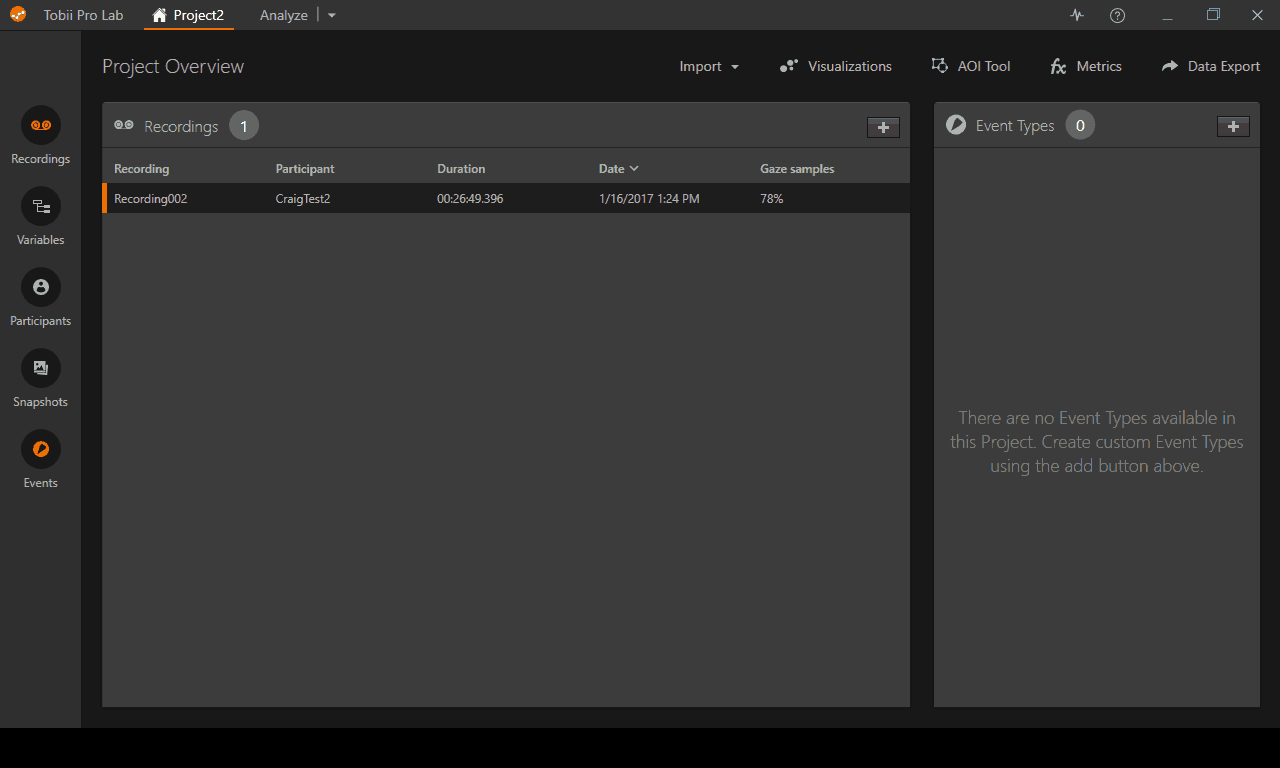
\includegraphics[width=1\textwidth]{images/02/prolab.png}
    \caption{TODO, má zmysel ukázať ako vyzerá softvér?}
    \label{img:lab}
\end{figure}

Keďže dodávaný softvér pre náš prípad nedokázal pomôcť s analýzou, potrebovali sme vytvoriť systém, ktorý dokáže sledovať reklamy z videa. % Na to je potrebné disponovať detektorom objektov. 

% tensorboard https://medium.com/mlearning-ai/remote-tensorboard-viewing-on-your-local-browser-b0dc5c5a634a     and     https://pytorch.org/docs/stable/tensorboard.html

\section{Detektor reklám}

V návrhu sme sa rozhodli použiť kombináciu YOLOv8 a Mapillary Vistas. Z celkového počtu obrázkov bolo anotovaných približne 20000 obrázkov s reklamou. Väčšina obrázkov je uložená vo vysokom rozlíšení 3312x2444, kde plocha označených reklám je často menšia ako 0,1\% z celej plochy obrázka. 

% veľké P? Python

YOLOv8 je možné nainštalovať a importovať ako balík pre python. Trénovanie sa dá spustiť pomocou jedného príkazu, kde sa špecifikujú všetky parametre. Pre prvotné trénovanie sme ponechali všetky parametre prednastavené. Na trénovanie sme mali k dispozícii školský server, ktorý má dve grafické karty NVIDIA GeForce RTX 3060, každá s 12 GB pamäte, CPU AMD Ryzen 9 5900X a 64 GB RAM.

%, ktorým nepomohlo ani drobné ladenie parametrov

Tréning skončil so slabými výsledkami. Predpokladali sme, že veľká chybovosť nastáva práve pri najmenšie označených reklamách. Preto sme dataset vytriedili a ponechali len také obrázky, kde reklamná plocha tvorila aspoň 0,1\% z obrázka. Počet obrázkov tým klesol pod 11000. Natrénovali sme hneď aj tretí model sme k vytriedeným obrázkom pridali ďalších 350 snímok, ktoré boli vystrihnuté z testovacích videí nahratých cez eyetracker. Každý tréning mal dataset rozdelený na tri časti v pomere 8:1:1 pre tréningovú, validačnú a testovaciu sadu.

\begin{table}
\centering
\begin{tabular}{ |c c c c c c c|  }
\hline
epochy & dávka & krok učenia & rozlíšenie & optimizer & dropout & váhy \\
\hline
128	  	& 16	& 0.01	& 640 & SGD & 0.0 & yolov8L \\
\hline
\end{tabular}
\caption{Hodnoty pre základné parametre pri trénovaní .}
\label{table:1}
\end{table}

Okrem vyhodnotenia výsledkov na testovacej sade sme si pripravili testovaciu vzorku obrázkov tvorenú z 250 snímok z experimentálneho merania. Výsledky troch modelov na testovacej sade a vzorke sú v tabuľke \ref{table:test}. Na vytváranie anotácií sme použili webovú aplikáciu Darwin v7labs \cite{v7}.

\begin{table}
\centering
\begin{tabular}{ |c c c c c|  }
\hline
model & precision & recall & mAP50 & mAP50-95 \\ 
\hline
\hline
\multicolumn{5}{|c|}{Tréningová sada} \\
\hline
M1  & 0.473	& 0.352	& 0.327	& 0.195 \\
M2  & 0.659 & 0.565 & 0.656 & 0.467 \\
M3  & 0.623 & 0.575 & 0.636 & 0.456 \\
\hline
\hline
 \multicolumn{5}{|c|}{Testovacia vzorka} \\
\hline
M1  & 0.473	& 0.352	& 0.327	& 0.195 \\
M2  & 0.659 & 0.565 & 0.656 & 0.467 \\
M3  & 0.623 & 0.575 & 0.636 & 0.456 \\
\hline
\end{tabular}
\caption{TODO, môžu byť výsledky v takejto kombinovanej tabuľke?}
\label{table:test}
\end{table}

% Vyhodnotenie na testovacej vzorke sme robili z toho dôvodu, že sme vedeli, že potrebujeme vytvoriť model, ktorý bude schopný detegovať reklamy z nahrávok čo najlepšie.
Pre pokračovanie sme zvolili model M3, pretože dosahoval najlepšie výsledky na testovacej vzorke. Na sledovanie reklám vo videách sme pripravili metódy z kapitoly XY. Výsledky sme najskôr vyhodnotili iba pozorovaním, pretože sme nemali skutočne pravdivé údaje. Na priblíženie sa ku skutočne pravdivým údajom sme zvolili spôsob natrénovať pomocný model, ktorý bol trénovaný zo snímok vystrihnutých z nahrávok experimentu. Reklamy zo snímok sme najskôr dali detegovať pomocou modelu M3. Získané označenia sme potom pridali do aplikácie Darwin v7labs a následne opravili vzniknuté chyby. Takýto dataset dosiahol veľkosť takmer 1000 obrázkov. Pomocný model na testovacej vzorke dosahoval presnosť X percent (TODO dopočítať).

\subsubsection{Sledovanie reklám}

S pomocným modelom sme pre sledovanie reklám vytvorili testovaciu sadu pre 20 reklám z prvého videa. Ani pomocný model nedokázal reklamy sledovať reklamy presne, preto sme opäť upravili vzniknuté chyby. Testovacia sada pre sledovanie reklám bola uložená vo formáte uvedenom na obrázku XY. Každá snímka, na ktorej sa nachádzala reklama bola zapísaná v samostatnom riadku s niekoľkými hodnotami. V poradí zľava - poradie snímku, referencia reklamy, x a y súradnica ľavého horného rohu reklamy, šírka a výška reklamy.

Porovnanie sledovacích metód s modelom M3 na testovacej sade pre sledovanie reklám je zapísané v tabuľke XY.

\begin{table}
\centering
\begin{tabular}{|c c c c c c c c c|} 
 \hline
metóda & HOTA & DetPr & DetRe & DetA & AssPr & AssRe & AssA & LocA \\ [0.5ex] 
 \hline
deep & 39.152 & 63.357 & 54.578 & 42.673 & 70.841 & 42.888 & 35.937 & 88.932\\ [0.1ex]
oc & 37.936 & 58.479 & 54.554 & 40.455 & 74.731 & 42.579 & 35.638 & 88.581\\ [0.1ex]
byte & 27.760 & 37.434 & 34.147 & 22.085 & 57.887 & 47.258 & 34.957 & 88.027\\ [0.1ex]
bot & 27.141 & 40.139 & 38.162 & 24.812 & 40.389 & 56.746 & 29.729 & 87.301\\ [0.1ex]
 \hline
\end{tabular}
\caption{HOTA.}
\label{table:1}
\end{table}

Pre účely dosiahnuť čo najviac snímok s reklamou sme metódy nastavili tak, aby mali čo najväčšiu hodnotu pre recall. Samozrejme sa tým znížila celková presnosť sledovania (HOTA), ale to v podstate nebolo dôležité, pretože sme vedeli, že pred počítaním fixácií potrebujeme každú reklamu označiť rovnakou referenciou v každom videu.

Metódu s vysokou citlivosťou sme použili na detekciu reklám z každej nahrávky z merania. Museli sme opraviť dve chyby, falošne pozitívne detekcie a správne priradenie referencie. Prakticky to znamenalo, že sme si dali vykresliť všetky detekcie do každého videa s uvedenou referenciou. Pokiaľ išlo o správnu detekciu reklamy, priradili sme jej referenciu, ktorá bola rovnaké pre každé video. Dosiahli sme tak dve veci jednou ranou a získané výsledky sme považovali za skutočne pravdivé údaje.

Porovnanie sledovacích metód s modelom M3 na nových údajoch je zapísané v tabuľke XY. Vyhodnotená bola iba polovica jázd, pretože ...

\begin{table}
\centering
\begin{tabular}{|c c c c c c c c c|}
 \hline
jazda & HOTA & DetPr & DetRe & DetA & AssPr & AssRe & AssA & LocA \\ [0.5ex] 
 \hline
1 & 39.152 & 63.357 & 54.578 & 42.673 & 70.841 & 42.888 & 35.937 & 88.932\\ [0.1ex]
2 & 37.936 & 58.479 & 54.554 & 40.455 & 74.731 & 42.579 & 35.638 & 88.581\\ [0.1ex]
3 & 27.760 & 37.434 & 34.147 & 22.085 & 57.887 & 47.258 & 34.957 & 88.027\\ [0.1ex]
5 & 27.141 & 40.139 & 38.162 & 24.812 & 40.389 & 56.746 & 29.729 & 87.301\\ [0.1ex]
~ & 33.843 & 51.285 & 46.888 & 33.210 & 42.917 & 67.840 & 34.528 & 88.368\\ [0.1ex]
 \hline
\end{tabular}
\caption{HOTA.}
\label{table:1}
\end{table}

\subsection{Významnosť reklám}

Z údajov sme dokázali vypočítať počet snímok, na ktoré sa vodič pozrel a podľa toho prideliť významnosť pre každú reklamu. V tomto bode sme zistili, že pohľady boli zaznamenaná s 50/s a video záznam 25/s. Preto sme pre každú snímku mali dva pohľady. Naopak, tak ako bolo naznačené v tabuľke X, niektoré snímky nemali pohľad. Pokiaľ išlo jeden-dva výpadky po sebe, tak sme sa hodnotu snažili dopočítať. Inak sme snímok vynechali. Tu sú výsledky ...

% todo pridať obrázok, kde je fixácia
% todo pridať obrázok, kde sa trajektória
% todo pridať obrázok, kde je graf z tréningu

\begin{table}
\centering
\begin{tabular}{|c c c c|}
 \hline
 CATEGORY &	RANGE &	COUNTER &	AVG CARS \\ [0.5ex] 
 \hline
NONE &	0 ms &	27 &	- \\ [0.1ex]
SHORT &	1-29 ms &	66 &	2.95 \\ [0.1ex]
MEDIUM &	30-59 ms &	18 &	5.11 \\ [0.1ex]
LONG &	60+ ms &	3 &	2 \\ [0.1ex]
TOTAL &	0-72 ms	& 114	& - \\ [0.1ex]
 \hline
\end{tabular}
\caption{TODO.}
\label{table:1}
\end{table}

\subsection{Klasifikácia reklamy}

% yolov5 (minuloročný model), yolov7, yolov8
% optimalizácia hyperparametre, Under/over-fitting
% augmentacia pred trenovanim, pri testovani (Test time augmentation)

% porovnanie precision a recall pre detector vs tracker
% can object tracking improve object detection?

% Yes, object tracking can improve object detection. Object tracking can be used to refine the object detection process by providing additional information about the location and movement of objects in a video stream. By tracking objects across multiple frames, object tracking algorithms can help to reduce false positives and false negatives in the object detection process. For example, if an object detection algorithm detects an object in one frame but fails to detect it in the next frame, an object tracking algorithm can use the object's previous position and movement to predict its location in the current frame. This can help to reduce the number of false negatives and improve the accuracy of the object detection algorithm. Additionally, object tracking can be used to filter out false positives in the object detection process. By tracking an object across multiple frames, an object tracking algorithm can verify that the object is indeed present and is not just a false positive detection. This can help to improve the precision of the object detection algorithm. Overall, object tracking and object detection are complementary techniques that can be used together to improve the accuracy and robustness of computer vision systems.

% kategorizácia
% spôsob
% výsledky

% porovnať chybosť kategorizácie, kebyže sa to počíta zo standardného modelu

% klasifikácia
% features
% výsledky

% porovnať chybosť klasifikácie, kebyže sa to počíta zo standardného modelu